% \begin{figure}[h!]
%     \centering
%     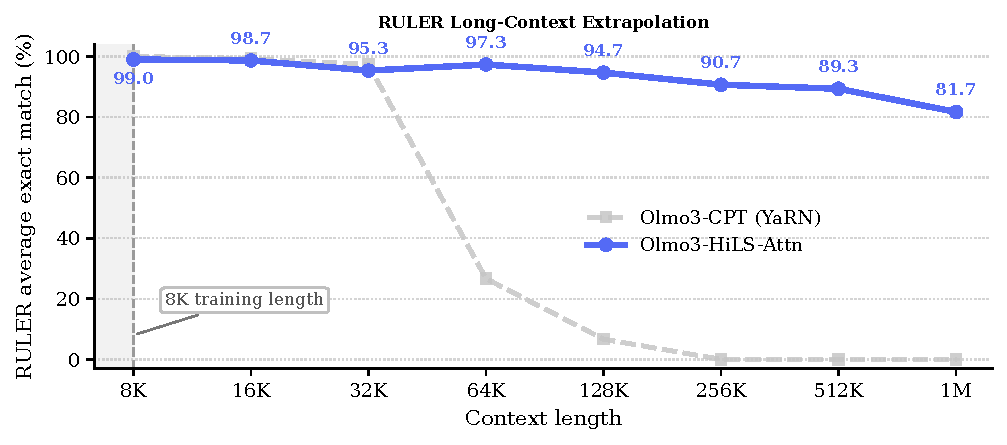
\includegraphics[width=0.95\linewidth]{data/ruler_extrapolation.pdf}
%     \includegraphics[width=0.95\linewidth]{data/longbench_v1_bar_comparison.pdf}
%     \includegraphics[width=0.95\linewidth]{data/non_ruler_bar_comparison.pdf}
%     \caption{Converting full attention to HiLS-Attention with only 50B continued-training tokens improves inference efficiency without sacrificing performance. Within the 8K training length, HiLS-Attention maintains comparable—and even slightly better—performance than full attention, while demonstrating strong long-context extrapolation advantages beyond the training length.}
% % TODO: OLMo3-8B ==> OLMo3-7B
%     \label{fig:placeholder}
% \end{figure}

\begin{figure}[h!]
    % \centering
    % 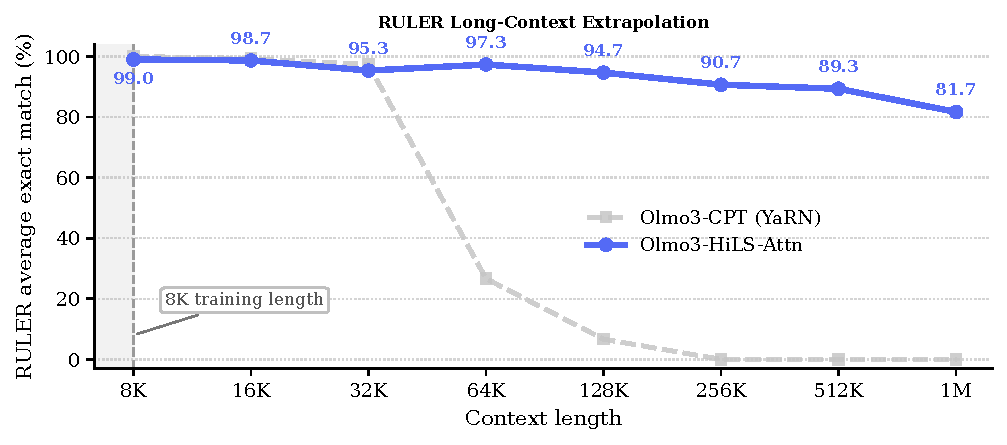
\includegraphics[width=0.92\linewidth]{data/ruler_extrapolation.pdf}
    % \label{fig_ruler_extra}
    % \par\vspace{-0.45em}
    % {\small\textbf{(a)}}
    % \par\vspace{0.3em}

    
    % \begin{minipage}[t]{0.345\linewidth}
    %     \vspace{0pt}
    %     \centering
    %     \vspace{0.18\linewidth}
    %     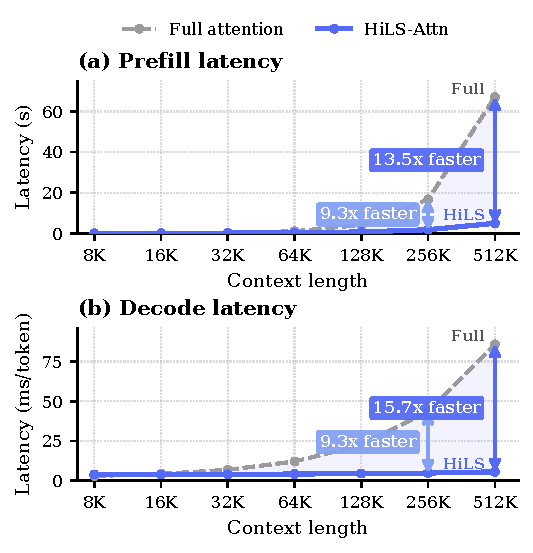
\includegraphics[width=\linewidth]{data/efficiency_speedup.pdf}
    %     \par\vspace{-0.45em}
    %     {\small\textbf{(b)}}
    % \end{minipage}
    % \hfill
    % \begin{minipage}[t]{0.645\linewidth}
    %     \vspace{0pt}
    %     \centering
    %     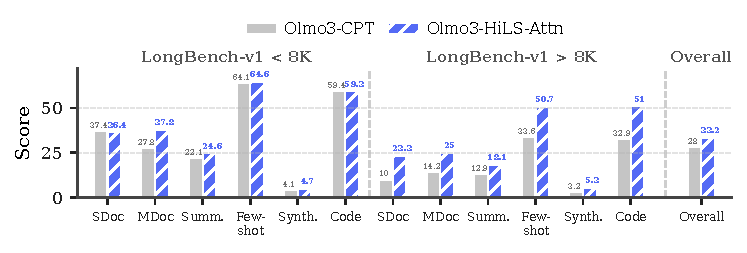
\includegraphics[width=\linewidth]{data/longbench_v1.pdf}
    %     \par\vspace{-0.45em}
    %     {\small\textbf{(c)}}
    %     \vspace{0.15em}

    %     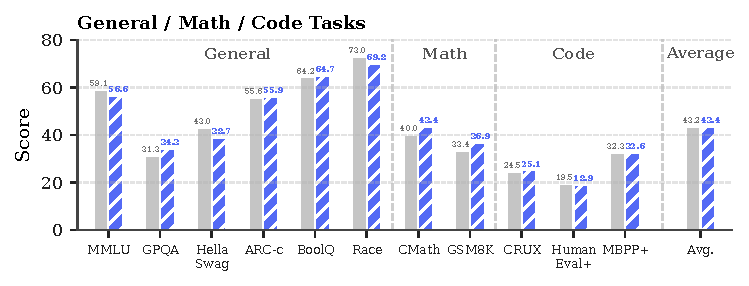
\includegraphics[width=\linewidth]{data/general_tasks.pdf}
    %     \par\vspace{-0.45em}
    %     {\small\textbf{(d)}}
    % \end{minipage}


    % \centering
    
    \begin{subfigure}[b]{0.9\linewidth}
        \centering
        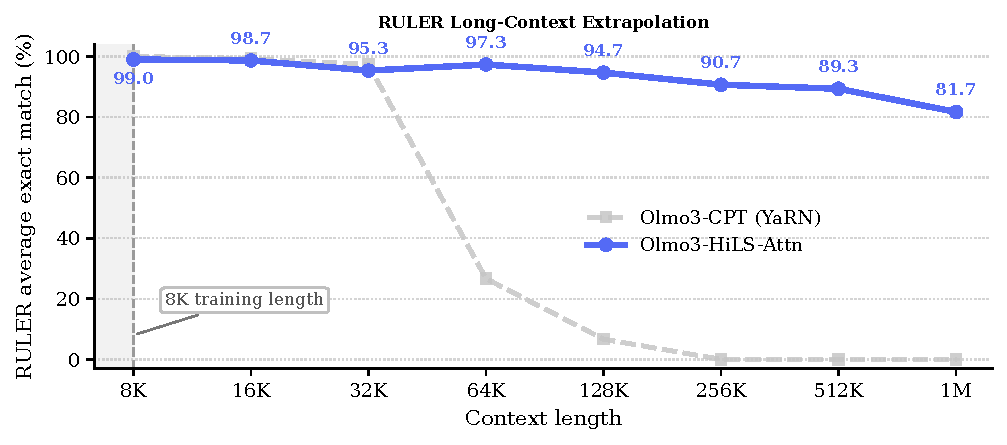
\includegraphics[width=\linewidth]{data/ruler_extrapolation.pdf}
        \caption{}
        \label{fig:ruler_extra}
    \end{subfigure}
    \begin{subfigure}[b]{0.4\linewidth}
        \centering
        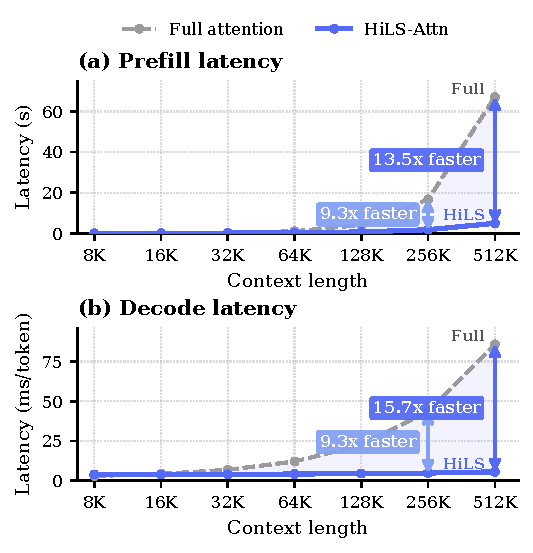
\includegraphics[width=\textwidth]{data/efficiency_speedup.pdf}
        \caption{}
        \label{fig:efficiency_speedup}
    \end{subfigure}
    \begin{minipage}[b]{0.55\linewidth}
        \centering
        \begin{subfigure}{\linewidth}
            \centering
            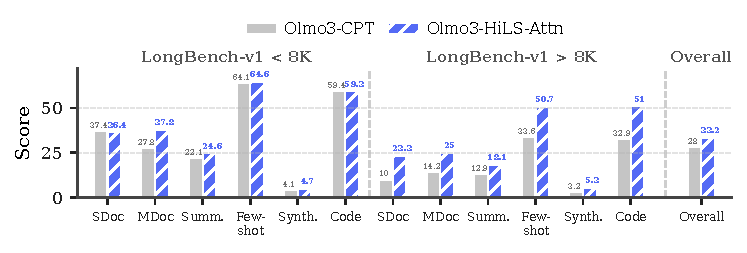
\includegraphics[width=\linewidth]{data/longbench_v1.pdf}
            \caption{}
            \label{fig:longbench_v1}
        \end{subfigure}
        \begin{subfigure}{\linewidth}
            \centering
            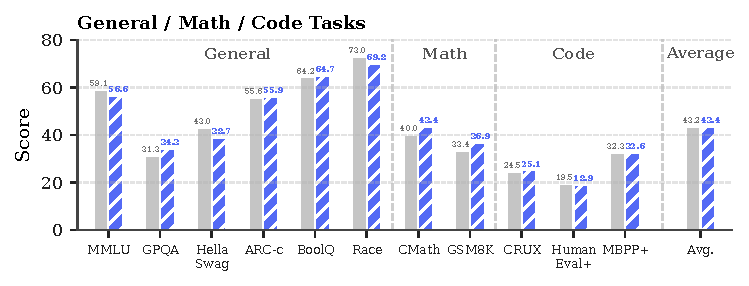
\includegraphics[width=\linewidth]{data/general_tasks.pdf}
            \caption{}
            \label{fig:general_task}
        \end{subfigure}
    \end{minipage}

    \caption{After only 50B continued-training tokens, HiLS-Attention inherits the capability of full attention while bringing two key advantages: \textit{strong ultra-long context extrapolation} beyond the YaRN-extended 4$\times$ length (Fig.~\ref{fig:ruler_extra}) and \textit{faster inference} (Fig.~\ref{fig:efficiency_speedup}) . Meanwhile, it preserves comparable performance for  short- and medium-context tasks, within both the original training length and the YaRN-extrapolated range (Fig.~\ref{fig:longbench_v1} \& \ref{fig:general_task}). %\leo{the result in subfig (c) does not show significant performance advantage of HiLS-attention over baseline. Any other more significant experiment results can be put here?}
    }
    %Converting full attention to HiLS-Attention with only 50B continued-training tokens improves inference efficiency without sacrificing performance(b)(c)(d). Within the 8K training length, HiLS-Attention even achieves slightly better performance than full attention (b)(c), while demonstrating strong long-context extrapolation advantages beyond the training length (a)(b). \leo{Keep the size of these subfigures same if their conclusion are equally important; otherwise, introduce conclusion from subfig (a) first since it is put most significant.}}
    \label{fig:main_results}
\end{figure}
